% ---- pg-600 （书页 588） ----

\begin{mvtable}
\mvtabcap{表 2\quad 学生 $t$ 分布百分位点}
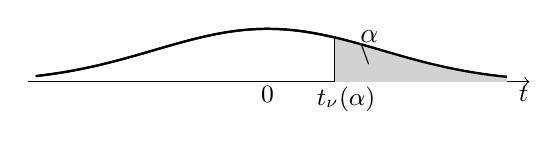
\begin{tikzpicture}[x=0.95cm,y=1.6cm]
% ---- 坐标轴 ----
\draw[->] (-3.2,0) -- (3.5,0);
% ---- t 分布密度曲线（近似） ----
\draw[thick,domain=-3.1:3.2,samples=100]
  plot (\x,{0.42*exp(-0.28*\x*\x)*(1+0.06*\x*\x)});
% ---- 曲线下右侧阴影区 ----
\fill[gray!35]
  (0.9,0) -- plot[domain=0.9:3.2,samples=60]
  (\x,{0.42*exp(-0.28*\x*\x)*(1+0.06*\x*\x)}) -- (3.2,0) -- cycle;
\draw[thick,domain=-3.1:3.2,samples=100]
  plot (\x,{0.42*exp(-0.28*\x*\x)*(1+0.06*\x*\x)});
% ---- t 处竖线 ----
\draw (0.9,0) -- (0.9,{0.42*exp(-0.28*0.81)*(1+0.06*0.81)});
% ---- 标注 ----
\draw (1.25,0.30) -- (1.35,0.14);
\node[inner sep=1pt] at (1.36,0.36) {$\alpha$};
% ---- 轴标签 ----
\node[below,inner sep=1pt,font=\small] at (0,-0.01) {$0$};
\node[below,inner sep=1pt,font=\small] at (1.05,-0.01) {$t_{\nu}(\alpha)$};
\node[below,inner sep=1pt,font=\small] at (3.42,-0.01) {$t$};
\end{tikzpicture}

{\zihao{6}
\begin{tabular}{r|*{9}{r}}
\toprule
\makecell{d. f.\\$\nu$} & \multicolumn{9}{c}{$\alpha$}\\
\cmidrule(lr){2-10}
& 0.250 & 0.100 & 0.050 & 0.025 & 0.010 & 0.00833 & 0.00625 & 0.005 & 0.0025\\
\midrule
1 & 1.000 & 3.078 & 6.314 & 12.706 & 31.821 & 38.190 & 50.923 & 63.657 & 127.321\\
2 & 0.816 & 1.886 & 2.920 & 4.303 & 6.965 & 7.649 & 8.860 & 9.925 & 14.089\\
3 & 0.765 & 1.638 & 2.353 & 3.182 & 4.541 & 4.857 & 5.392 & 5.841 & 7.453\\
4 & 0.741 & 1.533 & 2.132 & 2.776 & 3.747 & 3.961 & 4.315 & 4.604 & 5.598\\
5 & 0.727 & 1.476 & 2.015 & 2.571 & 3.365 & 3.534 & 3.810 & 4.032 & 4.773\\
6 & 0.718 & 1.440 & 1.943 & 2.447 & 3.143 & 3.287 & 3.521 & 3.707 & 4.317\\
7 & 0.711 & 1.415 & 1.895 & 2.365 & 2.998 & 3.128 & 3.335 & 3.499 & 4.029\\
8 & 0.706 & 1.397 & 1.860 & 2.306 & 2.896 & 3.016 & 3.206 & 3.355 & 3.833\\
9 & 0.703 & 1.383 & 1.833 & 2.262 & 2.821 & 2.933 & 3.111 & 3.250 & 3.690\\
10 & 0.700 & 1.372 & 1.812 & 2.228 & 2.764 & 2.870 & 3.038 & 3.169 & 3.581\\
11 & 0.697 & 1.363 & 1.796 & 2.201 & 2.718 & 2.820 & 2.981 & 3.106 & 3.497\\
12 & 0.695 & 1.356 & 1.782 & 2.179 & 2.681 & 2.779 & 2.934 & 3.055 & 3.428\\
13 & 0.694 & 1.350 & 1.771 & 2.160 & 2.650 & 2.746 & 2.896 & 3.012 & 3.372\\
14 & 0.692 & 1.345 & 1.761 & 2.145 & 2.624 & 2.718 & 2.864 & 2.977 & 3.326\\
15 & 0.691 & 1.341 & 1.753 & 2.131 & 2.602 & 2.694 & 2.837 & 2.947 & 3.286\\
16 & 0.690 & 1.337 & 1.746 & 2.120 & 2.583 & 2.673 & 2.813 & 2.921 & 3.252\\
17 & 0.689 & 1.333 & 1.740 & 2.110 & 2.567 & 2.655 & 2.793 & 2.898 & 3.222\\
18 & 0.688 & 1.330 & 1.734 & 2.101 & 2.552 & 2.639 & 2.775 & 2.878 & 3.197\\
19 & 0.688 & 1.328 & 1.729 & 2.093 & 2.539 & 2.625 & 2.759 & 2.861 & 3.174\\
20 & 0.687 & 1.325 & 1.725 & 2.086 & 2.528 & 2.613 & 2.744 & 2.845 & 3.153\\
21 & 0.686 & 1.323 & 1.721 & 2.080 & 2.518 & 2.601 & 2.732 & 2.831 & 3.135\\
22 & 0.686 & 1.321 & 1.717 & 2.074 & 2.508 & 2.591 & 2.720 & 2.819 & 3.119\\
23 & 0.685 & 1.319 & 1.714 & 2.069 & 2.500 & 2.582 & 2.710 & 2.807 & 3.104\\
24 & 0.685 & 1.318 & 1.711 & 2.064 & 2.492 & 2.574 & 2.700 & 2.797 & 3.091\\
25 & 0.684 & 1.316 & 1.708 & 2.060 & 2.485 & 2.566 & 2.692 & 2.787 & 3.078\\
26 & 0.684 & 1.315 & 1.706 & 2.056 & 2.479 & 2.559 & 2.684 & 2.779 & 3.067\\
27 & 0.684 & 1.314 & 1.703 & 2.052 & 2.473 & 2.552 & 2.676 & 2.771 & 3.057\\
28 & 0.683 & 1.313 & 1.701 & 2.048 & 2.467 & 2.546 & 2.669 & 2.763 & 3.047\\
29 & 0.683 & 1.311 & 1.699 & 2.045 & 2.462 & 2.541 & 2.663 & 2.756 & 3.038\\
30 & 0.683 & 1.310 & 1.697 & 2.042 & 2.457 & 2.536 & 2.657 & 2.750 & 3.030\\
40 & 0.681 & 1.303 & 1.684 & 2.021 & 2.423 & 2.499 & 2.616 & 2.704 & 2.971\\
60 & 0.679 & 1.296 & 1.671 & 2.000 & 2.390 & 2.463 & 2.575 & 2.660 & 2.915\\
120 & 0.677 & 1.289 & 1.658 & 1.980 & 2.358 & 2.428 & 2.536 & 2.617 & 2.860\\
$\infty$ & 0.674 & 1.282 & 1.645 & 1.960 & 2.326 & 2.394 & 2.498 & 2.576 & 2.813\\
\bottomrule
\end{tabular}}
\end{mvtable}
